\section{Results} \label{sec:results}
We plugged in the optimization \label{eq:opt} in an interactive freeform editing system. Our system computes an arrangement of curves from an input of polyline curves using CGAL's arrangement model \cite{cgal,cgal_arr1,cgal_arr2} and solves the the symmetric indefinite  linear systems \eqref{eq:linear_system} using Pardiso \cite{PARDISO1,PARDISO2,PARDISO3}. Our editing system supports setting handle based positional constraints (\figref{fig:teaser}, \figref{fig:multiple_crease_patterns}, and the second and last model from the left at \figref{fig:folded_and_not_folded}), constraining a crease curve by specifying its curvature and torsion in a curve constrained flow (\figref{fig:folded_and_not_folded}, \figref{fig:MV_bias_modeling}), and prescribing a sparse set of dihedral angles along crease points (\figref{fig:dihedral_editing}). \figref{fig:MV_bias_modeling} is the only figure where a mountain/valley assignment was given as input. The curve constrained positional constraints as well as the dihedral angles were interpolated for improved quality (see \figref{fig:homotopy_curve}). To maintain interactivity in handle based editing tasks we run a fixed number of SQP iterations per frame, which we set to $5$. Our system is able to handle interactive models of meshes with around $2,000$ vertices \MiR{some of the results with the curve constrained flows are bigger, and also the annulus was used by "pairing" vertices, so not interactive}. We refer the reader to our supplementary video for further results, including interactive editing examples. 

\begin{figure} [h]
	\centering
	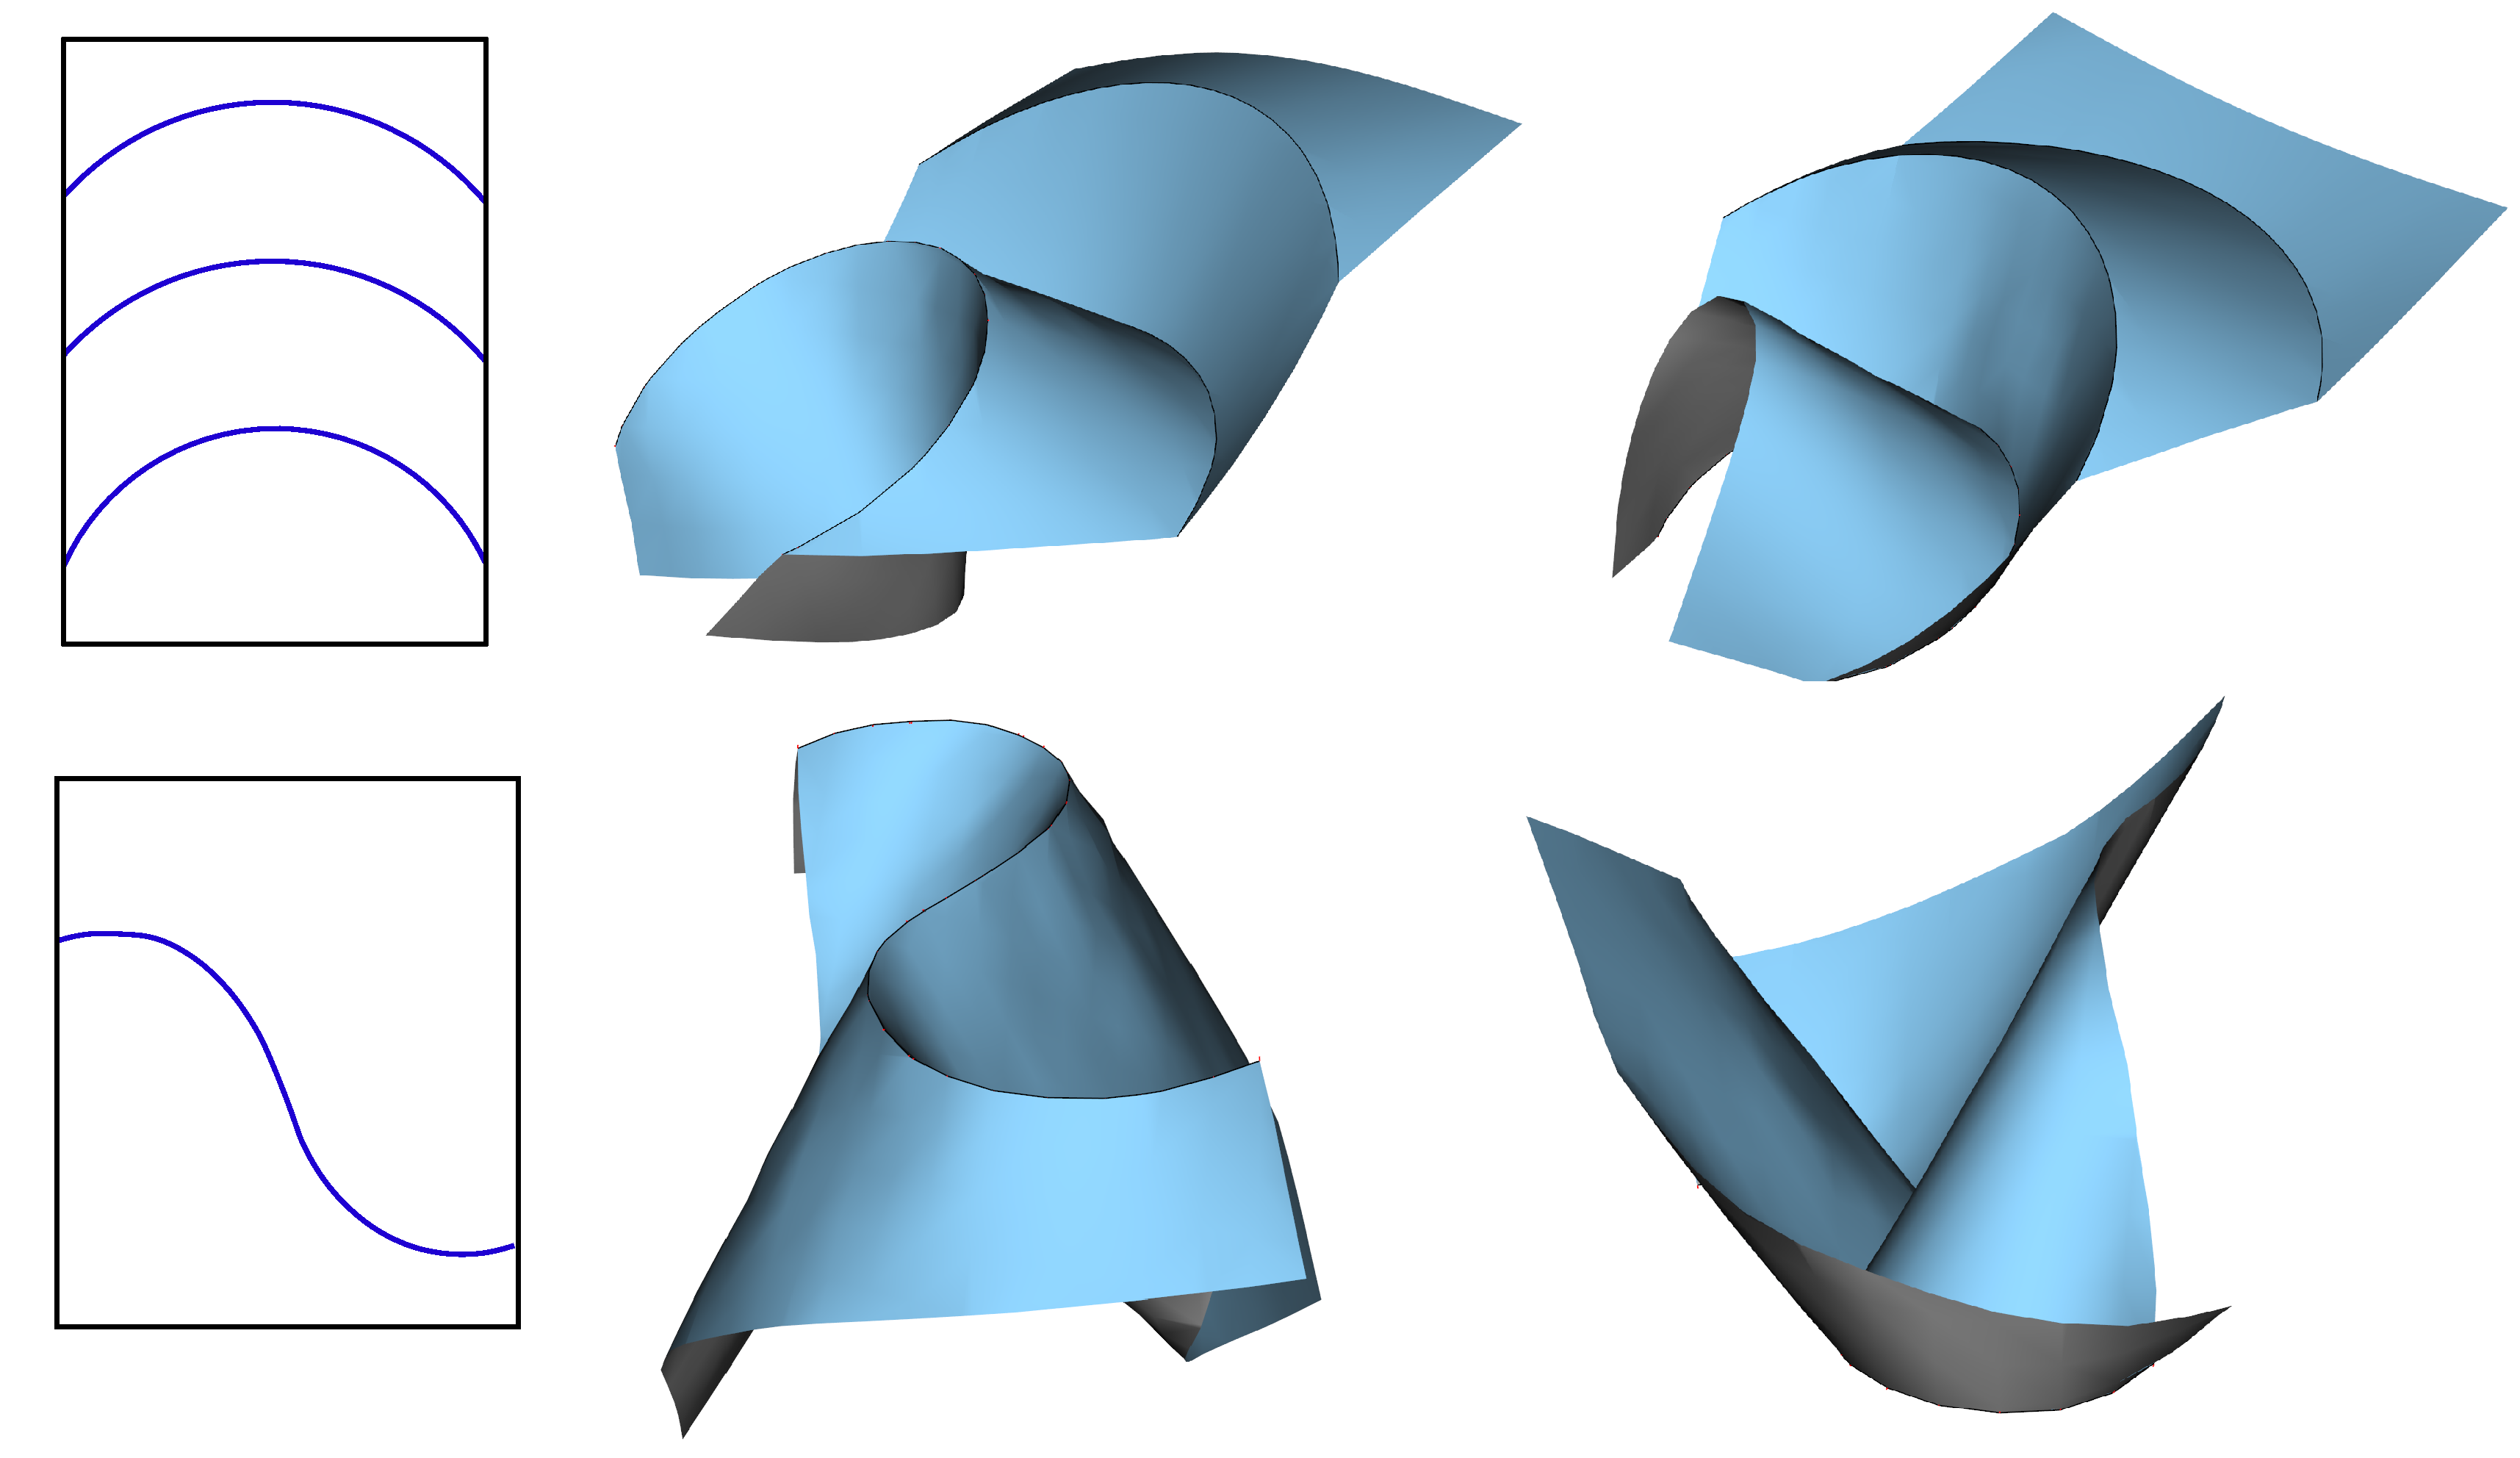
\includegraphics[width=\linewidth]{figures/MV_bias_modeling}
	\caption{Using the optional mountain valley input (\secref{sec:MV_assignments}) on a single crease curve. Each crease pattern was deformed with the same positional constraints, induced by a curve constrained flow, but with a different mountain/valley assignment along one fold, enforced by \eqref{eq:mountain_valley}. In the lower banana shaped model the rest of the mountain/valley assignments are then uniquely determined.}
	\label{fig:MV_bias_modeling}
\end{figure}

\begin{figure} [h]
	\centering
	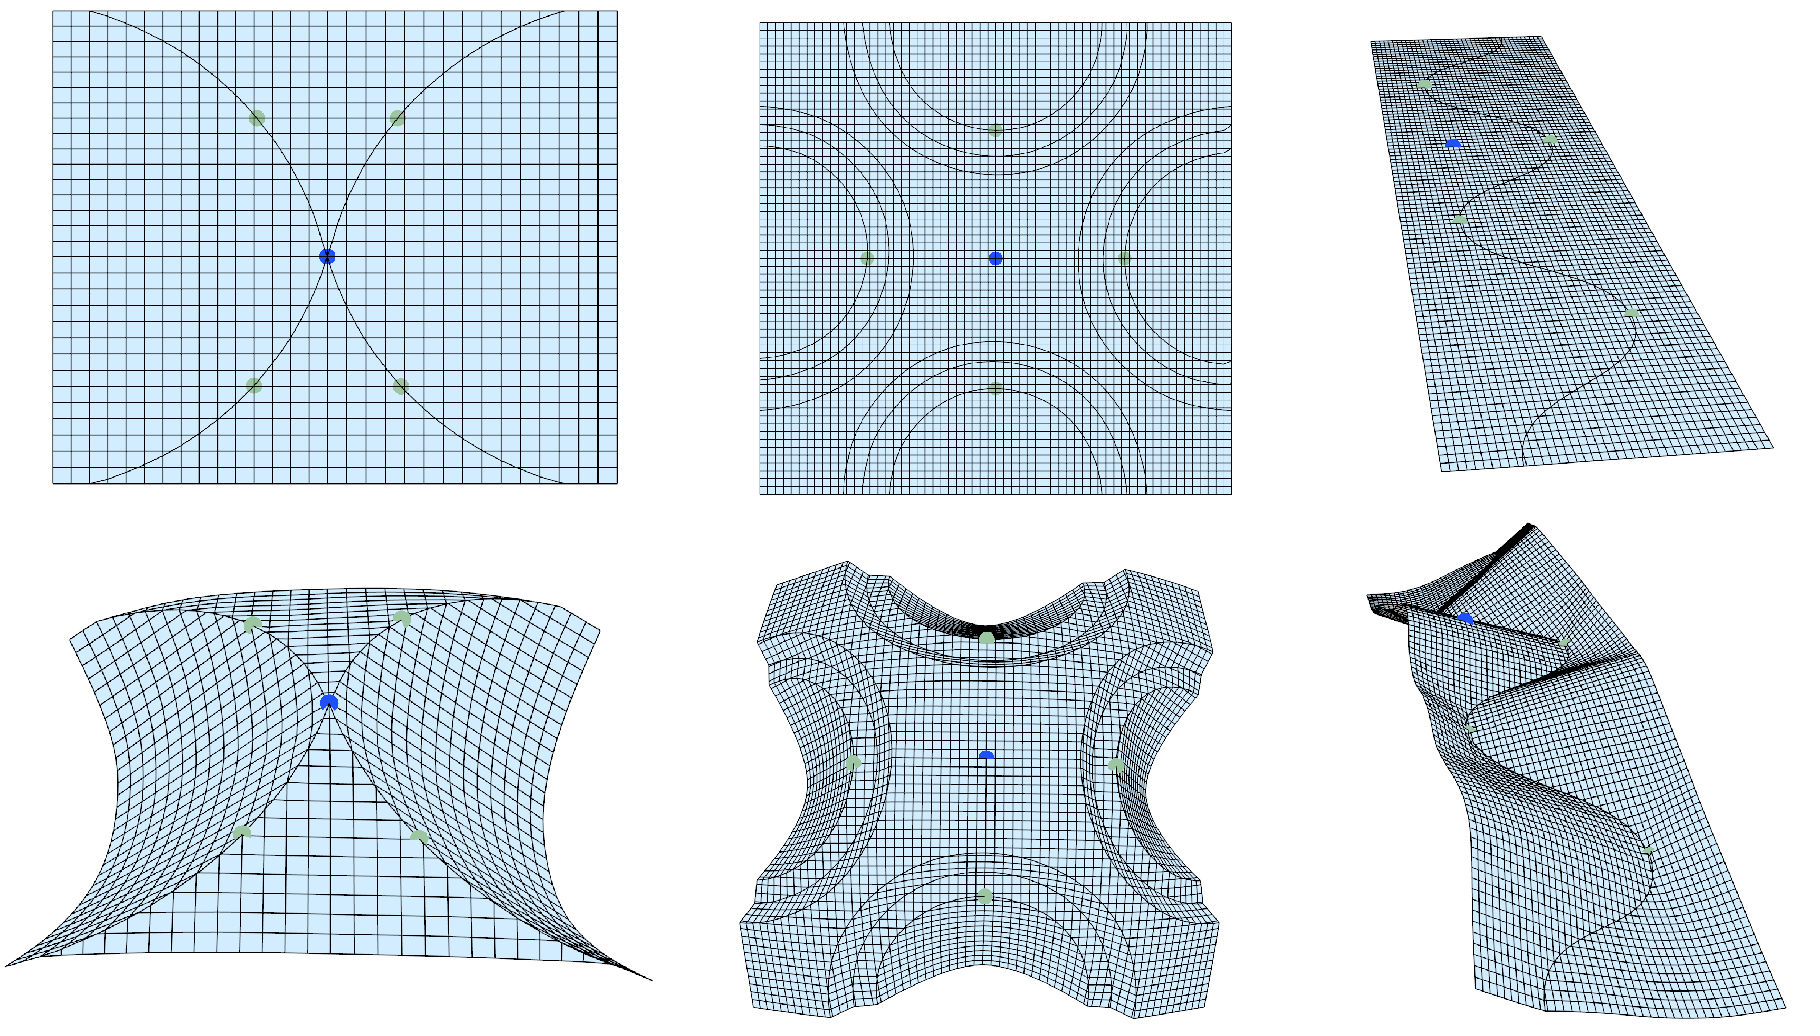
\includegraphics[width=\linewidth]{figures/dihedral_editing}
	\caption{Using the optional folding angle assignments (\secref{sec:folding_angle}) on a spare set of crease points. These examples were deformed by constraining the folding angle of a set of points (green), without specifying their folding orientation, and by setting a single positional constraint (blue).}
	\label{fig:dihedral_editing}
\end{figure}